\documentclass[12pt,letterpaper]{article}

\usepackage{arxiv}

\usepackage[utf8]{inputenc} % allow utf-8 input
\usepackage[T1]{fontenc}    % use 8-bit T1 fonts
\usepackage{hyperref}       % hyperlinks
\usepackage{url}            % simple URL typesetting
\usepackage{booktabs}       % professional-quality tables
\usepackage{amsfonts}       % blackboard math symbols
\usepackage{nicefrac}       % compact symbols for 1/2, etc.
\usepackage{microtype}      % microtypography
\usepackage{lipsum}
\usepackage{graphicx}	% Including figure files
\usepackage{mathtools}  %loads amsmath as well
\usepackage{amssymb}	% Extra maths symbols
\usepackage[english]{babel}
\usepackage{float}
\usepackage{bm}
\usepackage{indentfirst}
\usepackage{tikz}
\usetikzlibrary{positioning}
\usepackage{pgfplots}
\usepackage{color,soul}
%\pgfplotsset{compat=1.12}
\definecolor{mygray}{RGB}{125,125,125}
\definecolor{myred}{RGB}{255,60,60}
\definecolor{myblue}{RGB}{60,60,255}
\renewcommand{\arraystretch}{1.2}

% potential journals:
    % journal of computational physics
    % computers and fluids
    % international journal for numerical methods in fluids
    % aiaa
    % journal of fluid mechanics

\title{A Multiresolution Scheme Featuring Fully Adaptive Blocks for Simulating Reactive Flows}

\author{
  Brandon Gusto\\
  Department of Scientific Computing\\
  Florida State University\\
  Tallahassee, FL 32306 \\
  \texttt{bgusto@fsu.edu} \\
  %% examples of more authors
  \And
  Tomasz Plewa \\
  Department of Scientific Computing\\
  Florida State University\\
  Tallahassee, FL 32306 \\
  \texttt{tplewa@fsu.edu} \\
}

\begin{document}
\maketitle

\begin{abstract}
    We present a generalization of Harten's original multiresolution scheme for
    simulating reactive flows on logically rectangular block-structured adaptive
    mesh refinement (AMR) grids in one and two dimensions. The scheme addresses
    a major shortcoming of tree-based AMR codes, which is the creation of blocks
    with a low filling factor; that is, many cells in such a block are resolved
    beyond the desired error tolerance, necessitating excessive computational
    resources.  To overcome this issue, we introduce a multiresolution
    representation of the solution, not only to adapt the grid but also to
    adaptively compute fluxes and sources on each block. The scheme recycles
    regularity information obtained by the multiresolution grid adaptation in
    order to select flux and source calculations which may be accurately
    replaced by interpolation from the multiresolution basis. A block which
    employs this scheme is denoted as a fully adaptive block (FAB).  The error
    introduced by this approximation is shown to be of the same order as the
    local truncation error of the reconstruction scheme. Thus the rate of
    convergence of the underlying spatial reconstruction scheme is preserved.
    Additionally with respect to parallel applications, the multiresolution
    transform and computation of fluxes and sources on FABs is asynchronous,
    requiring only one synchronization step which is equivalent to the filling
    of ghost cells for each block. The efficiency of the scheme is demonstrated
    using several one and two-dimensional problems.
\end{abstract}

% keywords can be removed
\keywords{Multiresolution \and Adaptive Mesh Refinement \and Conservation Laws}

\section{Introduction}

    % paragraph introduces the need for spatially adaptive grids
    Fluid flows are often characterized by disparate spatial and temporal length
    scales. Certain features such as turbulence or shocks necessitate
    significantly higher resolution than smooth regions of the flow.  In
    reacting flows, combustion fronts often act in highly localized regions, and
    on very small time scales. Naturally, intense effort has gone into the
    development of methods which employ a multi-scale or adaptive strategy to
    accurately simulate such flows without over-resolving smooth areas of the
    domain.

    % paragraph introducing adaptive mesh refinement as a concept
    The most popular strategy to accurately capture regions of interest in fluid
    simulations is to introduce a non-uniform spatial grid, with higher
    resolution in regions of interest.  Methods which introduce a hierarchy of
    nested grid resolutions are generally described as adaptive mesh refinement
    (AMR) methods. AMR methods rely on estimates of the local truncation error (LTE)
    of the numerical scheme to determine regions where refinement is necessary for solution
    accuracy. Several strategies to approximate the LTE are used (\hl{list
    methods}).
    %\cite{Berger1984}.  Alternative methods include
    %feature-based refinement, and evaluation of gradient information (references
    %here).

    % talk about block-structured AMR
    Regarding the implementation of AMR methods on large parallel computers,
    certain engineering realities have neccessitated the reduction in
    granularity of the adaptive refinement. To use a single computational cell
    as the unit for refinement (i.e. cell-based refinement) introduces a number
    of costly compromises. Firstly, such an adapted grid requires the
    reconstruction method of choice to utilize nonuniform stencils, requiring
    increased computational resources. More significantly, the cell-based
    refinement requires extremely costly data traversal. Traversing tree space
    requires an average $\mathcal{O}(n^d)$ (\hl{confirm this?}) operations. Thus
    most AMR codes make use of some type of block-based approach. Tree-based
    block-structured codes, where each block consists of a fixed number of
    cells, are a very popular choice. These types of approaches are implemented
    in a number of AMR libraries including Paramesh (\hl{cite}), p4est
    (\hl{cite}, and others. This approach allows for simple mesh management
    procedures, and scales well for very large number of processors in parallel.

    % paragraph reviews the work of harten and multiresolution methods
    Alternate approaches to dynamic grid adaptation based on wavelet theory have
    become popular in recent years. The first such effort was introduced in a
    seminal paper by Harten \cite{harten1994}, where a multiresolution
    representation of the discrete solution on a uniform grid was used for
    adaptively computing the divergence of the flux within a finite volume
    framework. Rather than adapt the grid by truncating the wavelet basis, the
    idea was to accelerate the computation of high-order essentially
    non-oscillatory (ENO) schemes using the multiresolution information. Fluxes
    in smooth regions were interpolated from fluxes obtained at interfaces
    corresponding to coarser grid levels. The original scheme was applied solely
    to hyperbolic conservation laws, but was then expanded by Bihari et. al. to
    two-dimensional simulations in (\hl{citation}), followed by the inclusion of
    viscous terms in (\hl{citation}), and then tp source terms in the context of
    reactive flows in (\hl{citation}). These works retained the original flavor
    of Harten's scheme, which was to represent the discrete solution on a
    uniform grid, but uses a multiresolution representation of the solution to
    identify regions where flux (and source term) computations may be avoided.
    The multiresolution transform is obtained by using average-interpolating
    wavelets as basis functions.

    % review the multiresolution-adaptive papers
    Although Harten's original scheme was intended to be an alternative to
    spatially non-uniform grid adaptation, a series of papers have since
    reintroduced this concept of non-uniform grids within the MR framework. Thus
    the AMR approach has been redeveloped but with the refinement criterion
    defined by the MR representation rather than with the traditional metrics
    mentioned previously. The first fully adaptive scheme was presented by Cohen
    et. al. to study hyperbolic conservation laws in two dimensions in
    (\hl{cite}).

\section{Governing Equations and Finite Volume Discretization}

    % describe merging block-structured AMR with Harten's scheme
    In the present work we are interested in numerically solving conservation
    laws of the form
    \begin{equation}
    \begin{cases}
      u_{t} + f(u)_{x} = s(u) \\    
      u(x,0) = u_{0}(x),
    \end{cases}
    \label{claw}
    \end{equation} where $u$ represents a conserved quantity, $f(u)$ is the flux
    function, and $s(u)$ is a source term. For the sake of presentation, we let
    the scalar equation (\ref{claw}) stand in for the more complicated systems
    of conversation laws which will be the focus of our applications.  In the
    finite volume formulation, the solution $u(x,t)$ is approximated by volume
    averages defined within each cell $I_{i} = \left[ x_{i}-\frac{h}{2},
    x_{i}+\frac{h}{2} \right]$ in the computational domain.  The cell width $h$
    is determined by the number of cells, $N$, and the size of the domain
    $\Omega \in \left[a,b\right]$.  The cell averages are given by
    \begin{equation}
        \overline{u}_{i}(t) = \frac{1}{h} \int_{x_{i-1/2}}^{x_{i+1/2}} u(\xi,t) d \xi,
    \end{equation}
    where for convenience we use $i \pm 1/2$ in the subscripts to
    indicate the left and right interfaces of the target cell (i.e.
    $x_{i+1/2} =
    x_{i} + \frac{h}{2}$). The governing equations are cast into the
    semi-discrete conservative form,
    \begin{equation}
        \frac{d\overline{u}_{i}(t)}{dt} = -\frac{1}{h} \left( \hat{f}_{i+1/2} -
        \hat{f}_{i-1/2} \right),
        \label{ode}
    \end{equation}
    where the numerical flux is evaluated as
    \begin{equation}
        \hat{f}_{i + 1/2} = \hat{f}(u^{-}_{i+1/2}, u^{+}_{i+1/2}).
    \end{equation}
    In the present work, the reconstruction method of choice is a fifth-order
    weighted essentially non-oscillatory (WENO) scheme.

    \subsection{WENO Reconstruction Scheme}

    \subsection{Time Integration}
     
        % define evolution operator as in domingues2008
        Once the system of ordinary differential equations (\ref{ode}) is
        established, the objective is to integrate them forward in time. In our
        implementation we use a second-order explicit Runge-Kutta scheme to
        advance. This is summarized by
        \begin{equation}
            \bm{u}^{n+1} = \bm{E} \bm{u}^{n},
        \end{equation}
        where $\bm{E}$ represents the nonlinear evolution operator, and codifies the
        temporal and spatial discretizations.

\section{Harten's Multiresolution Scheme}

    % describe overview of transform, and average-interpolating wavelets
    The average-interpolating multiresolution approach is based on a hierarchy
    of nested discretizations on the domain of interest $\Omega$. In the case of
    a one-dimensional, uniformly spaced grid, the hierarchy is defined by
    \begin{equation}
        \mathcal{G}^{l} = \left\{ x_{i}^{l} \right\}_{i=0}^{N^{l}}, \text{ }
        \text{ } \text{ } \text{ } x_{i}^{l} = i \cdot h^{l}, \text{ }
        \text{ } h^{l} = 2^{L-l} \cdot h^{L}, \text{ } \text{ } N^{l} = N^{L}
        / 2^{L-l},
    \end{equation}
    where the finest grid is denoted by $\mathcal{G}^{L}$, and on any arbitrary
    level $l$, the cell width is $h^{l}$, and the number of cells is $N^{l}$.
    Given a vector of discrete cell averages $\bm{u}^{L}$ at the finest
    resolution, the multiresolution representation is obtained by the following
    operations:
    \begin{enumerate}
        \item[] \textit{Split:} The cells at grid level $l$ are split into two
            sets, even and odd.
        \item[] \textit{Project:} The cells at level $l$ are projected, or
            coarsened by means of volume averaging onto the coarser grid level
            $l-1$.
        \item[] \textit{Predict}: A stencil of odd cell averages at level $l$ are predicted
                by an average-interpolating polynomial based on cells at level
                $l-1$.
    \end{enumerate}
    The splitting of cells is done simply according to the cell index. The
    projection is defined by a linear operator $P_{l}^{l-1}$, which performs the
    mapping $P_{l}^{l-1} : \bm{u}_{l} \rightarrow \bm{u_{l-1}}$. The projection
    preserves averages at the finer level.  maps the vector $\bm{u}^{l}$ to
    $\bm{u}^{l-1}$. This is done using average-interpolating polynomials to
    predict, based on a stencil of cell-averages at one grid level, the cell
    averages at one finer level of resolution. This process is done in a
    principled way, and defines the forward wavelet transform (also known as
    \textit{encoding}). The transform consists of two steps: Once the prediction
    step is complete, the regularity information about the underlying function
    sampled at level $l$ has been obtained. The scheme is explored in more
    detail by first examining the grid hierarchy needed for the multiresolution
    representation of the data.

    \subsection*{Grid Hierarchy}


    \subsection*{Forward Transform}

        % describe the prediction operator, and detail coefficients
        The forward transform provides regularity information about the function
        underlying the fine-grid data. The transform procedure can be succinctly
        written in terms of a matrix-vector operation to yield the
        multiresolution representation of the data, $u_{MR}^{0}$, as
        \begin{equation}
            \bm{u}_{M}^{l} = \bm{M}^{l} \bm{u}^{l} = \left( \bm{d}^{l+1}, \bm{d}^{l+2},
            \dots, \bm{d}^{l+L}; \bm{u}^{L} \right)^{T}.
        \end{equation}
        Here the multiresolution operator $\bm{M}$ contains the prediction
        operator for each
        \begin{equation}
            \tilde{u}_{2i+1}^{l-1} \approx u_{i}^{l} - \sum_{p=1}^{s}
            \gamma_{p} \left( u^{l}_{i-p} - u^{l}_{i+p} \right).
        \end{equation}
        In Table (1) the coefficients are shown for several average-interpolating stencils
        \begin{table}
            \centering
            \begin{tabular}{|l|l|l|l|}
            \hline
                & $\gamma_{1}$ & $\gamma_{2}$ & $\gamma_{3}$ \\ \hline
                $s=1$ & $1/8$ & 0 & 0 \\ \hline
                $s=2$ & $-22/128$ & $3/128$ & 0 \\ \hline
            \end{tabular}
            \caption{Coefficients for cell-average interpolation in the prediction step.}
        \end{table}
        The detail coefficients are then computed as
        \begin{equation}
            d^{l}_{i} = u^{l-1}_{2i+1} - \tilde{u}^{l-1}_{2i+1}.
        \end{equation}
        These steps are illustrated in Figure (2).

    the difference information is
    easily obtained by comparing the odd-indexed cell-averages at level $l$ with
    their predicted values.

    % illustration of parallel fwt 
    \begin{figure}[H]
        \center
        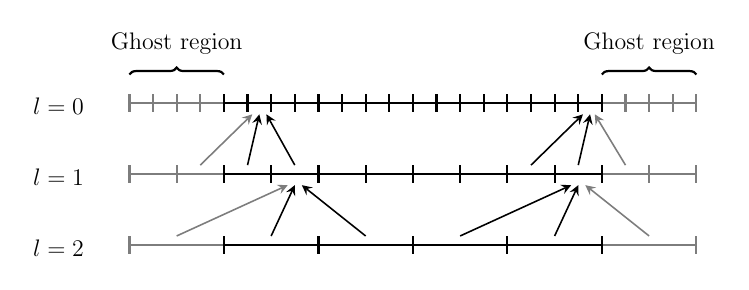
\begin{tikzpicture}[thick,scale=0.3, every node/.style={scale=0.6}]

    % variables
    \def\xl{-8.0}
    \def\xr{8.0}
    \def\y{0.0}
    \def\yy{-3.0}
    \def\yyy{-6.0}
    \def\ts{0.75}
    \def\op{0.35}
    \def\fx{0.15}
    
    % draw ghost cells
    \draw [mygray] (\xl-4,\y+\ts/2) --(\xr+4,\y+\ts/2);
    \draw [mygray] (\xl-4,\yy+\ts/2) --(\xr+4,\yy+\ts/2);
    \draw [mygray] (\xl-4,\yyy+\ts/2) --(\xr+4,\yyy+\ts/2);
    \draw [mygray] (\xl-1.0,\y) --(\xl-1.0,\y+\ts);
    \draw [mygray] (\xr+1.0,\y) --(\xr+1.0,\y+\ts);
    \draw [mygray] (\xl-2.0,\y) --(\xl-2.0,\y+\ts);
    \draw [mygray] (\xr+2.0,\y) --(\xr+2.0,\y+\ts);
    \draw [mygray] (\xl-3.0,\y) --(\xl-3.0,\y+\ts);
    \draw [mygray] (\xr+3.0,\y) --(\xr+3.0,\y+\ts);
    \draw [mygray] (\xl-4.0,\y) --(\xl-4.0,\y+\ts);
    \draw [mygray] (\xr+4.0,\y) --(\xr+4.0,\y+\ts);

    % ghost cells at level l=1
    \draw [mygray] (\xl-2.0,\yy) --(\xl-2.0,\yy+\ts);
    \draw [mygray] (\xr+2.0,\yy) --(\xr+2.0,\yy+\ts);
    \draw [mygray] (\xl-4.0,\yy) --(\xl-4.0,\yy+\ts);
    \draw [mygray] (\xr+4.0,\yy) --(\xr+4.0,\yy+\ts);

    % level l=2
    \draw [mygray] (\xl-4.0,\yyy) --(\xl-4.0,\yyy+\ts);
    \draw [mygray] (\xr+4.0,\yyy) --(\xr+4.0,\yyy+\ts);

    % draw grids
    \draw (\xl,\y+\ts/2) --(\xr,\y+\ts/2);
    \draw (\xl,\yy+\ts/2) --(\xr,\yy+\ts/2);
    \draw (\xl,\yyy+\ts/2) --(\xr,\yyy+\ts/2);
    
    % draw cells for max level
    \draw (\xl,\y) --(\xl,\y+\ts);
    \draw (\xl+1.0,\y) --(\xl+1.0,\y+\ts);
    \draw (\xl+2.0,\y) --(\xl+2.0,\y+\ts);
    \draw (\xl+3.0,\y) --(\xl+3.0,\y+\ts);
    \draw (\xl+4.0,\y) --(\xl+4.0,\y+\ts);
    \draw (\xl+5.0,\y) --(\xl+5.0,\y+\ts);
    \draw (\xl+6.0,\y) --(\xl+6.0,\y+\ts);
    \draw (\xl+7.0,\y) --(\xl+7.0,\y+\ts);
    \draw (\xl+8.0,\y) --(\xl+8.0,\y+\ts);
    \draw (\xl+9.0,\y) --(\xl+9.0,\y+\ts);
    \draw (\xl+10.0,\y) --(\xl+10.0,\y+\ts);
    \draw (\xl+11.0,\y) --(\xl+11.0,\y+\ts);
    \draw (\xl+12.0,\y) --(\xl+12.0,\y+\ts);
    \draw (\xl+13.0,\y) --(\xl+13.0,\y+\ts);
    \draw (\xl+14.0,\y) --(\xl+14.0,\y+\ts);
    \draw (\xl+15.0,\y) --(\xl+15.0,\y+\ts);
    \draw (\xl+16.0,\y) --(\xl+16.0,\y+\ts);
    
    % lower level cells
    \draw (\xl,\yy) --(\xl,\yy+\ts);
    \draw (\xl+2.0,\yy) --(\xl+2.0,\yy+\ts);
    \draw (\xl+4.0,\yy) --(\xl+4.0,\yy+\ts);
    \draw (\xl+6.0,\yy) --(\xl+6.0,\yy+\ts);
    \draw (\xl+8.0,\yy) --(\xl+8.0,\yy+\ts);
    \draw (\xl+10.0,\yy) --(\xl+10.0,\yy+\ts);
    \draw (\xl+12.0,\yy) --(\xl+12.0,\yy+\ts);
    \draw (\xl+14.0,\yy) --(\xl+14.0,\yy+\ts);
    \draw (\xl+16.0,\yy) --(\xl+16.0,\yy+\ts);
    
    % even lower level cells
    \draw (\xl,\yyy) --(\xl,\yyy+\ts);
    \draw (\xl+4.0,\yyy) --(\xl+4.0,\yyy+\ts);
    \draw (\xl+8.0,\yyy) --(\xl+8.0,\yyy+\ts);
    \draw (\xl+12.0,\yyy) --(\xl+12.0,\yyy+\ts);
    \draw (\xl+16.0,\yyy) --(\xl+16.0,\yyy+\ts);
 
    % arrows indicating flux interpolation dependency
    \draw[->,line width=0.2mm,>=stealth] (\xr-3,\yy+\ts) -- (\xr-0.8,\y-0.1);
    \draw[->,line width=0.2mm,>=stealth] (\xr-1,\yy+\ts) -- (\xr-0.5,\y-0.1);
    \draw[mygray,->,line width=0.2mm,>=stealth] (\xr+1,\yy+\ts) -- (\xr-0.3,\y-0.1);

    \draw[->,line width=0.2mm,>=stealth] (\xr-6,\yyy+\ts) -- (\xr-1.3,\yy-0.1);
    \draw[->,line width=0.2mm,>=stealth] (\xr-2,\yyy+\ts) -- (\xr-1,\yy-0.1);
    \draw[mygray,->,line width=0.2mm,>=stealth] (\xr+2,\yyy+\ts) -- (\xr-0.7,\yy-0.1);

    \draw[mygray,->,line width=0.2mm,>=stealth] (\xl-1,\yy+\ts) -- (\xl+1.2,\y-0.1);
    \draw[->,line width=0.2mm,>=stealth] (\xl+1,\yy+\ts) -- (\xl+1.5,\y-0.1);
    \draw[->,line width=0.2mm,>=stealth] (\xl+3,\yy+\ts) -- (\xl+1.8,\y-0.1);

    \draw[mygray,->,line width=0.2mm,>=stealth] (\xl-2,\yyy+\ts) -- (\xl+2.7,\yy-0.1);
    \draw[->,line width=0.2mm,>=stealth] (\xl+2,\yyy+\ts) -- (\xl+3,\yy-0.1);
    \draw[->,line width=0.2mm,>=stealth] (\xl+6,\yyy+\ts) -- (\xl+3.3,\yy-0.1);

    % curly brace
    \draw[decoration={brace,raise=5pt},decorate]
        (\xr,\y+1.0) -- node[above=10pt] {\Large Ghost region}(\xr+4.0,\y+1.0);
    \draw[decoration={brace,raise=5pt},decorate]
        (\xl-4.0,\y+1.0) -- node[above=10pt] {\Large Ghost region}(\xl,\y+1.0);

    % nodes
    \node at (\xl-7.0,\y+0.25) {\Large $l=0$};
    \node at (\xl-7.0,\yy+0.25) {\Large $l=1$};
    \node at (\xl-7.0,\yyy+0.25) {\Large $l=2$};

\end{tikzpicture}

        \caption{A block of consisting of $N^{0} = 16$ cells is shown. Four
        ghost cells are included on each end of the block, allowing the
        multiresolution decomposition to descend two levels (to grid level
        $l=2$). Interpolation stencils for the computation of detail
        coefficients at levels $l=1, l=2$ are shown, indicating the need for ghost cells.}
    \end{figure}

\subsection*{Inverse Transform}

    % 
    
\subsection*{Calculation of Fluxes and Sources}
    Once the detail coefficients have been obtained, the MR scheme
    proceeds by setting a threshold $\epsilon$ and truncating coefficients
    which have an absolute value below the threshold. Lastly, the inverse
    transform then starts from grid $l=L$ and at each interface either
    computes fluxes using the fine-grid scheme, or interpolates them using
    the MR basis. The fluxes are interpolated by
    \begin{align}
        & \tilde{f}_{2i+1}^{l-1} \approx \sum_{p=1}^{s+1} \alpha_{p} \left(
        \hat{f}^{l}_{i-p+1} + \hat{f}^{l}_{i+p} \right),
    \end{align}
    where the interpolants are of degree $2s+1$. The coefficients for
    various degrees of polynomial interpolants are shown in Table (ref).
    \begin{table}
        \centering
        \begin{tabular}{|l|l|l|l|}
        \hline
            & $\alpha_{1}$ & $\alpha_{2}$ & $\alpha_{3}$ \\ \hline
            $s=0$ & 1/2 & 0 & 0 \\ \hline
            $s=1$ & 9/16 & -1/16 & 0 \\ \hline
        \end{tabular}
        \caption{Coefficients for cell-average interpolation in the prediction step.}
    \end{table}
    The process repeats until all fluxes are either computed or
    interpolated on the fine grid $l=0$.

    \subsection*{Error Analysis}

        % describe choice of epsilon

\section{Asynchronous Fully Adaptive Block Scheme}

    % two main issues: no jump greater than one refinement level, and no
    % incomplete trees

    % illustration amr block tree structure
    \begin{figure}[H]
        \center
        \input{amr_tree.tex}
        \caption{}
    \end{figure}

    % pseudocode of algorithm

    % illustration of parallel issue
    \begin{figure}[H]
        \center
        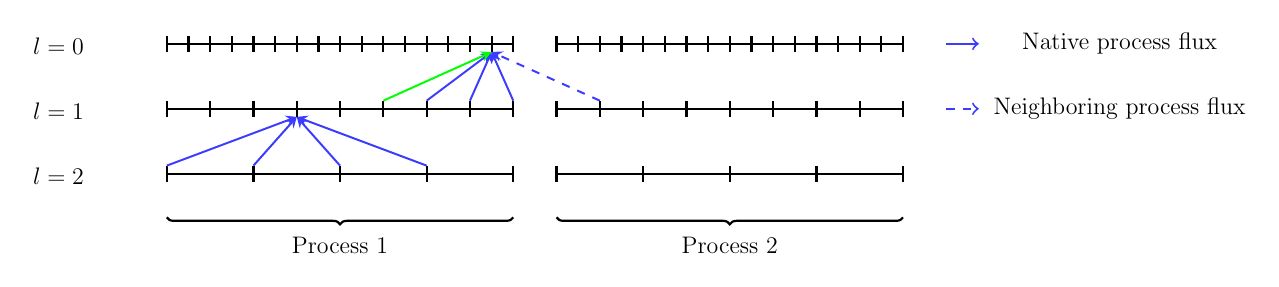
\begin{tikzpicture}[thick,scale=0.275, every node/.style={scale=0.6}]

    % variables
    \def\xl{-8.0}
    \def\xr{8.0}
    \def\y{0.0}
    \def\yy{-3.0}
    \def\yyy{-6.0}
    \def\ts{0.75}
    \def\op{0.35}
    \def\fx{0.15}
    
    % draw grids
    \draw (\xl,\y+\ts/2) --(\xr,\y+\ts/2);
    \draw (\xl,\yy+\ts/2) --(\xr,\yy+\ts/2);
    \draw (\xl,\yyy+\ts/2) --(\xr,\yyy+\ts/2);
    
    % draw cells for max level
    \draw (\xl,\y) --(\xl,\y+\ts);
    \draw (\xl+1.0,\y) --(\xl+1.0,\y+\ts);
    \draw (\xl+2.0,\y) --(\xl+2.0,\y+\ts);
    \draw (\xl+3.0,\y) --(\xl+3.0,\y+\ts);
    \draw (\xl+4.0,\y) --(\xl+4.0,\y+\ts);
    \draw (\xl+5.0,\y) --(\xl+5.0,\y+\ts);
    \draw (\xl+6.0,\y) --(\xl+6.0,\y+\ts);
    \draw (\xl+7.0,\y) --(\xl+7.0,\y+\ts);
    \draw (\xl+8.0,\y) --(\xl+8.0,\y+\ts);
    \draw (\xl+9.0,\y) --(\xl+9.0,\y+\ts);
    \draw (\xl+10.0,\y) --(\xl+10.0,\y+\ts);
    \draw (\xl+11.0,\y) --(\xl+11.0,\y+\ts);
    \draw (\xl+12.0,\y) --(\xl+12.0,\y+\ts);
    \draw (\xl+13.0,\y) --(\xl+13.0,\y+\ts);
    \draw (\xl+14.0,\y) --(\xl+14.0,\y+\ts);
    \draw (\xl+15.0,\y) --(\xl+15.0,\y+\ts);
    \draw (\xl+16.0,\y) --(\xl+16.0,\y+\ts);
    
    % lower level cells
    \draw (\xl,\yy) --(\xl,\yy+\ts);
    \draw (\xl+2.0,\yy) --(\xl+2.0,\yy+\ts);
    \draw (\xl+4.0,\yy) --(\xl+4.0,\yy+\ts);
    \draw (\xl+6.0,\yy) --(\xl+6.0,\yy+\ts);
    \draw (\xl+8.0,\yy) --(\xl+8.0,\yy+\ts);
    \draw (\xl+10.0,\yy) --(\xl+10.0,\yy+\ts);
    \draw (\xl+12.0,\yy) --(\xl+12.0,\yy+\ts);
    \draw (\xl+14.0,\yy) --(\xl+14.0,\yy+\ts);
    \draw (\xl+16.0,\yy) --(\xl+16.0,\yy+\ts);
    
    % even lower level cells
    \draw (\xl,\yyy) --(\xl,\yyy+\ts);
    \draw (\xl+4.0,\yyy) --(\xl+4.0,\yyy+\ts);
    \draw (\xl+8.0,\yyy) --(\xl+8.0,\yyy+\ts);
    \draw (\xl+12.0,\yyy) --(\xl+12.0,\yyy+\ts);
    \draw (\xl+16.0,\yyy) --(\xl+16.0,\yyy+\ts);
    
    % curly brace
    \draw[decoration={brace,mirror,raise=5pt},decorate]
        (\xl,\yyy-1.0) -- node[below=10pt] {\Large Process 1}(\xr,\yyy-1.0);

    % arrows indicating flux interpolation dependency
    \draw[myblue,->,line width=0.25mm,>=stealth] (\xr-4,\yy+\ts) -- (\xr-1,\y);
    \draw[myblue,->,line width=0.25mm,>=stealth] (\xr-2,\yy+\ts) -- (\xr-1,\y);
    \draw[myblue,->,line width=0.25mm,>=stealth] (\xr,\yy+\ts) -- (\xr-1,\y);
    \draw[myblue,dashed,->,line width=0.25mm,>=stealth] (\xr+4,\yy+\ts) -- (\xr-1,\y);
    \draw[green,->,line width=0.25mm,>=stealth] (\xr-6,\yy+\ts) -- (\xr-1,\y);

    \draw[myblue,->,line width=0.25mm,>=stealth] (\xr-16,\yyy+\ts) -- (\xr-10,\yy);
    \draw[myblue,->,line width=0.25mm,>=stealth] (\xr-12,\yyy+\ts) -- (\xr-10,\yy);
    \draw[myblue,->,line width=0.25mm,>=stealth] (\xr-8,\yyy+\ts) -- (\xr-10,\yy);
    \draw[myblue,->,line width=0.25mm,>=stealth] (\xr-4,\yyy+\ts) --(\xr-10,\yy);

    % nodes
    \node at (\xl-5.0,\y+0.25) {\Large $l=0$};
    \node at (\xl-5.0,\yy+0.25) {\Large $l=1$};
    \node at (\xl-5.0,\yyy+0.25) {\Large $l=2$};

    % draw process 2 grid
    \def\xl{10.0}
    \def\xr{26.0}
    \draw (\xl,\y+\ts/2) --(\xr,\y+\ts/2);
    \draw (\xl,\yy+\ts/2) --(\xr,\yy+\ts/2);
    \draw (\xl,\yyy+\ts/2) --(\xr,\yyy+\ts/2);
    
    % draw cells for max level
    \draw (\xl,\y) --(\xl,\y+\ts);
    \draw (\xl+1.0,\y) --(\xl+1.0,\y+\ts);
    \draw (\xl+2.0,\y) --(\xl+2.0,\y+\ts);
    \draw (\xl+3.0,\y) --(\xl+3.0,\y+\ts);
    \draw (\xl+4.0,\y) --(\xl+4.0,\y+\ts);
    \draw (\xl+5.0,\y) --(\xl+5.0,\y+\ts);
    \draw (\xl+6.0,\y) --(\xl+6.0,\y+\ts);
    \draw (\xl+7.0,\y) --(\xl+7.0,\y+\ts);
    \draw (\xl+8.0,\y) --(\xl+8.0,\y+\ts);
    \draw (\xl+9.0,\y) --(\xl+9.0,\y+\ts);
    \draw (\xl+10.0,\y) --(\xl+10.0,\y+\ts);
    \draw (\xl+11.0,\y) --(\xl+11.0,\y+\ts);
    \draw (\xl+12.0,\y) --(\xl+12.0,\y+\ts);
    \draw (\xl+13.0,\y) --(\xl+13.0,\y+\ts);
    \draw (\xl+14.0,\y) --(\xl+14.0,\y+\ts);
    \draw (\xl+15.0,\y) --(\xl+15.0,\y+\ts);
    \draw (\xl+16.0,\y) --(\xl+16.0,\y+\ts);
    
    % lower level cells
    \draw (\xl,\yy) --(\xl,\yy+\ts);
    \draw (\xl+2.0,\yy) --(\xl+2.0,\yy+\ts);
    \draw (\xl+4.0,\yy) --(\xl+4.0,\yy+\ts);
    \draw (\xl+6.0,\yy) --(\xl+6.0,\yy+\ts);
    \draw (\xl+8.0,\yy) --(\xl+8.0,\yy+\ts);
    \draw (\xl+10.0,\yy) --(\xl+10.0,\yy+\ts);
    \draw (\xl+12.0,\yy) --(\xl+12.0,\yy+\ts);
    \draw (\xl+14.0,\yy) --(\xl+14.0,\yy+\ts);
    \draw (\xl+16.0,\yy) --(\xl+16.0,\yy+\ts);
    
    % even lower level cells
    \draw (\xl,\yyy) --(\xl,\yyy+\ts);
    \draw (\xl+4.0,\yyy) --(\xl+4.0,\yyy+\ts);
    \draw (\xl+8.0,\yyy) --(\xl+8.0,\yyy+\ts);
    \draw (\xl+12.0,\yyy) --(\xl+12.0,\yyy+\ts);
    \draw (\xl+16.0,\yyy) --(\xl+16.0,\yyy+\ts);
    
    % curly brace
    \draw[decoration={brace,mirror,raise=5pt},decorate]
        (\xl,\yyy-1.0) -- node[below=10pt] {\Large Process 2}(\xr,\yyy-1.0);

    % legend
    \draw[myblue,->,line width=0.25mm] (\xr+2,\y+\ts/2) -- (\xr+3.5,\y+\ts/2);
    \draw[myblue,->,dashed,line width=0.25mm] (\xr+2,\yy+\ts/2) -- (\xr+3.5,\yy+\ts/2);
    \node at (\xr+10,\y+\ts/2) {\Large Native process flux};
    \node at (\xr+10,\yy+\ts/2) {\Large Neighboring process flux};

\end{tikzpicture}

       \caption{Two examples of flux interpolation on a hierarchy of grids
        on Process 1: one procedure requires flux data from the adjacent
        process, the other does not.}
    \end{figure}

    \subsection*{Buffer Region}

    \subsection*{Load Balancing}

\section{Numerical Results}

    \subsection*{Convergence Analysis}

        \begin{center}\vspace{1cm}
        \begin{tabular}{|l|l|l|l|l|l|l|l|l|}
        \hline
                   & \multicolumn{4}{l|}{$\epsilon = 0.0$}              & \multicolumn{4}{l|}{$\epsilon = 10^{-12}$}         \\ \hline
        grid cells & $L_{1}$ error & order & $L_{\infty}$ error & order & $L_{1}$ error & order & $L_{\infty}$ error & order \\ \hline
        16         &               &       &                    &       &               &       &                    &       \\ \hline
        32         &               &       &                    &       &               &       &                    &       \\ \hline
        64         &               &       &                    &       &               &       &                    &       \\ \hline
        128        &               &       &                    &       &               &       &                    &       \\ \hline
        256        &               &       &                    &       &               &       &                    &       \\ \hline
                   & \multicolumn{4}{l|}{$\epsilon = 10^{-6}$}          & \multicolumn{4}{l|}{$\epsilon = 10^{-4}$}          \\ \hline
        grid cells & $L_{1}$ error & order & $L_{\infty}$ error & order & $L_{1}$ error & order & $L_{\infty}$ error & order \\ \hline
        16         &               &       &                    &       &               &       &                    &       \\ \hline
        32         &               &       &                    &       &               &       &                    &       \\ \hline
        64         &               &       &                    &       &               &       &                    &       \\ \hline
        128        &               &       &                    &       &               &       &                    &       \\ \hline
        256        &               &       &                    &       &               &       &                    &       \\ \hline
        \end{tabular}
        \end{center}\vspace{1cm}

    \subsection*{Example}
    Using the inviscid flow assumption, the dynamics of compressible fluids are
    modeled using the reactive Euler equations \hl{add domain notation}
    \begin{equation}
       u_{t} + f(u)_{x}
       + g(u)_{y} = s(u),
        \label{goveq}
    \end{equation}
    where $u = \left( \rho, \rho u, \rho v, \rho w, E \right)^{T}$ is
    the state vector, the flux vectors are given by
    \begin{equation}
        f = 
    \begin{pmatrix}
    \rho u \\ \rho u^2 + p \\ \rho u v \\ \rho u w \\ u( E + p )
    \end{pmatrix}, \text{ } \text{ } \text{ }
        g = 
    \begin{pmatrix}
    \rho v \\ \rho u v \\ \rho v^2 + p \\ \rho v w \\ v( E + p )
    \end{pmatrix}, \text{ } \text{ } \text{ }
        h = 
    \begin{pmatrix}
    \rho w \\ \rho u w \\ \rho v w \\ \rho w^2 + p \\ w( E + p )
    \end{pmatrix},
    \end{equation}
    and $s(u)$ represents sources. The total energy per
    unit volume is given by
    \begin{equation*}
        E = \rho \left( \frac{1}{2} \mathbf{V}^{2} + e \right),
    \end{equation*}
    where $e$ is the internal energy and the kinetic energy contribution is
    \begin{equation*}
        \frac{1}{2} \mathbf{V}^{2} = \frac{1}{2} \mathbf{V}
        \cdot \mathbf{V} = \frac{1}{2} \left( u^2 + v^2 + w^2 \right).
    \end{equation*}
    The system of nonlinear equations is closed by an
    equation of state which is in general not derived from that of an ideal gas.

\section{Acknowledgements}

\appendix

\section{Multiresolution Analysis}

    % describe multiresolution analysis (sourced from tymczak2000)
    A multiresolution analysis (MRA) of the Lebesgue space
    $L^{2}(\mathbb{R})$ defines a sequence of nested approximation spaces.
    These spaces satisfy certain self-similarity properties in both space
    and scale. An MRA defines a sequence of closed subspaces $\{ \mathcal{V}_{j} : j \in
    \mathbb{Z} \}$ such that
    \begin{equation*}
        \mathcal{V}_{0} \subset \mathcal{V}_{1} \subset \mathcal{V}_{2} \subset \cdots
        \subset L^{2}.
    \end{equation*}
    The complement of $\mathcal{V}_{j} \in \mathcal{V}_{j+1}$ is defined by
    $\mathcal{W}_{j}$, known as the detail space. This relation is defined
    by a direct summation as
    \begin{equation*}
        \mathcal{V}_{j+1} = \mathcal{W}_{j} \oplus \mathcal{V}_{j}.
    \end{equation*}
    Considering successively finer approximation spaces yields for any
    arbitrary level $J$,
    \begin{equation*}
        \mathcal{V}_{J} = \mathcal{V}_0 \oplus \mathcal{W}_0 \oplus \mathcal{W}_1 \oplus \dots \oplus \mathcal{W}_{J-1}.
    \end{equation*}
    Thus fine-scale information on any arbitrary level $J$ is represented by
    the coarsest scale plus a series of differences at higher levels.
    Interested readers can refer to (\hl{cite}) for more details on the
    construction of the bi-orthogonal multiresolution analysis used.

    %, a real-valued scaling function
    %$\phi_{j}(x) \in V_{j}$ is defined which forms a basis,
    %\begin{equation*}
    %    V_{j} = \text{span} \left\{ \phi_{j}(x+k) : \forall k \right\}.
    %\end{equation*}

\section{Derivation of Prediction Operator in One-Dimension}

    % derivation of prediction operator
    We are interested in obtaining the difference between approximation spaces at varying levels of resolution. We 
    are given cell-averaged values as input data to our wavelet transform. This data is fed to the scheme at some arbitrary maximum
    resolution level $J$, and the wavelet transform produces details coefficients at each lower level until the coarsest level,
    $j=0$, is reached. The coefficients in this case are interchangeable with the cell-averages and are denoted by $c^{j}_{k}$,
    where the level of resolution is denoted by $j$, and the spatial index is denoted by $k$. We consider an interpolating
    polynomial $p(x)$ such that 
    \begin{align}
        c^{j}_{k-1} &= \int_{x^{j}_{k-1}}^{x^{j}_{k}} p(x) dx \\
        c^{j}_{k} &= \int_{x^{j}_{k}}^{x^{j}_{k+1}} p(x) dx \\
        c^{j}_{k+1} &= \int_{x^{j}_{k+1}}^{x^{j}_{k+2}} p(x) dx.
    \end{align}
    The polynomial $p(x)$ should then predict the finer cell-averages of cell $c^{j}_{k}$ as
    \begin{align}
        \hat{c}^{j+1}_{2k} &= 2 \int_{x^{j}_{k}}^{x^{j}_{k+1/2}} p(x) dx \\
        \hat{c}^{j+1}_{2k+1} &= 2 \int_{x^{j}_{k+1/2}}^{x^{j}_{k+1}} p(x) dx
    \end{align}
    At present, it may not be clear how to implement such a scheme on a computer. However this interpolation procedure
    can be cast in a more suitable form by introducing another polynomial, the integral of $p(x)$:
    \begin{equation}
        P(x) = \int_{0}^{x} p(y) dy.
    \end{equation}
    Now the problem is to interpolate the following data
    \begin{align}
        0 &= P(x^{j}_{k-1}) \\
        c^{j}_{k-1} &= P(x^{j}_{k}) \\
        c^{j}_{k-1} + c^{j}_{k} &= P(x^{j}_{k+1}) \\
        c^{j}_{k-1} + c^{j}_{k} + c^{j}_{k+1} &= P(x^{j}_{k+2}).
    \end{align}
    This can easily be done using Lagrange polynomials. Then the predictions are given in terms of $P(x)$ by
    \begin{align}
        \hat{c}^{j+1}_{2k} &= 2 \left( P(x^{j}_{k+1/2}) - P(x^{j}_{k}) \right) \\
        \hat{c}^{j+1}_{2k+1} &= 2 \left( P(x^{j}_{k+1}) - P(x^{j}_{k+1/2}) \right).
    \end{align}
    This interpolating polynomial is cast in the Lagrange form,
    \begin{equation}
    P(x) = \sum_{i=0}^{n} y_{i} l_{i}(x),
    \end{equation}
    where $y_{i}$ are the functional data, and $l_{i}(x)$ are the Lagrange polynomials. For $n=3$ these
    are given by
    \begin{align}
        l_{0}(x) &= \frac{x-x_1}{x_0-x_1} \frac{x-x_2}{x_0-x_2} \frac{x-x_3}{x_0-x_3} \\
        l_{1}(x) &= \frac{x-x_0}{x_1-x_0} \frac{x-x_2}{x_1-x_2} \frac{x-x_3}{x_1-x_3} \\
        l_{2}(x) &= \frac{x-x_0}{x_2-x_0} \frac{x-x_1}{x_2-x_1} \frac{x-x_3}{x_2-x_3} \\
        l_{3}(x) &= \frac{x-x_0}{x_3-x_0} \frac{x-x_1}{x_3-x_1} \frac{x-x_2}{x_3-x_2},
    \end{align}
    and the final interpolating polynomial is
    \begin{equation}
        P(x) = (0) l_{0}(x) + ( c^{j}_{k-1} ) l_{1}(x) + ( c^{j}_{k-1} + c^{j}_{k} ) l_{2}(x)
            + ( c^{j}_{k-1} + c^{j}_{k} + c^{j}_{k+1} ) l_{3}(x).
    \end{equation}
    Several evaluations are necessary in order to obtain the predictions. Using intervals of equal length, these values are
    \begin{align}
        P(x^{j}_{k}) &= c^{j}_{k-1} \\
        P(x^{j}_{k+1/2}) &= \frac{17}{16} c^{j}_{k-1} + \frac{1}{2} c^{j}_{k} - \frac{1}{16} c^{j}_{k+1} \\
        P(x^{j}_{k+1}) &= c^{j}_{k-1} + c^{j}_{k}.
    \end{align}
    Then the predictions of the cell-averages at the higher level of resolution are finally given by
    \begin{align}
        \hat{c}^{j+1}_{2k} & = c^{j}_{k} + \frac{1}{8} \left( c^{j}_{k-1} - c^{j}_{k+1} \right) \\
        \hat{c}^{j+1}_{2k+1} & = c^{j}_{k} - \frac{1}{8} \left( c^{j}_{k-1} - c^{j}_{k+1} \right).
    \end{align}
    This procedure could easily be extended to non-uniformly
    spaced intervals, giving different weights. Note that only the
    odd indices are counted because in the multiresolution scheme the
    data is initially split into even
    and odd signals. All data at level $j$ are just considered to
    be a copy of the even-index data at level $j+1$, whereas
    the odd-indexed data at level $j+1$ is what is predicted
    by even-indexed data at level $j+1$. Also important are the
    interpolants at the ends of the domain. Given below are the
    left and right predictions, respectively:
    \begin{align}
        \hat{c}^{j+1}_{2k+1} & = \frac{5}{8} c^{j}_{k}
        + \frac{1}{2} c^{j}_{k+1} - \frac{1}{8} c^{j}_{k+2} \\
        \hat{c}^{j+1}_{2k+1} & = \frac{1}{8} c^{j}_{k-2}
        - \frac{1}{2} c^{j}_{k-1} + \frac{11}{8} c^{j}_{k}.
    \end{align}

\bibliographystyle{unsrt}  
\bibliography{references}

\end{document}
